\documentclass[11pt]{article}
%\usepackage{fullpage}
\usepackage[top=2cm, bottom=1.5cm, left=1.5cm, right=1.5cm]{geometry}
\usepackage{amsmath,amsthm,amsfonts,amssymb,amscd}
\usepackage{xcolor}
\usepackage{graphicx}
\usepackage[utf8]{inputenc}
\usepackage[english]{babel}
\usepackage{fancyhdr}

\pagestyle{fancy}
\fancyhf{}
\fancyhead[LO]{Mechanics \& Relativity F3210}
\fancyhead[RO]{Workshop 3: Projectiles \& Uniform Circular Motion}
%\fancyfoot[CE,CO]{\leftmark}
%\fancyfoot[LE,RO]{\thepage}

%answers
\usepackage{etoolbox}
\providetoggle{answers}
\settoggle{answers}{false}

\newcommand\vect[1]{\underline{\mathbf{#1}}}
\newcommand\unitvect[1]{\hat{\boldsymbol{#1}}}

\begin{document}

\noindent
\textbf{\textcolor{red}{Please upload your solution to Problem 3 to canvas for marking after the workshop.}}\\

\section*{Problem 1}

A small ball rolls horizontally off the edge of a tabletop that is 1.20~m high. It strikes the floor at a point 1.52~m horizontally from the table edge.\\
(a) How long is the ball in the air?\\
(b) What is its speed at the instant it leaves the table?

\iftoggle{answers}{
\vspace{1cm}
\noindent
SOLUTION:\\

}{}


\section*{Problem 2}

When a large star becomes a supernova, its core may be compressed so tightly that it becomes a neutron star, with a radius of about 20~km (about the size of the San Francisco area). If a neutron star rotates once every second:\\
(a) What is the speed of a particle on the star's equator?\\
(b) What is the magnitude of the particle's centripetal acceleration?\\
(c) If the neutron star rotates faster, do the answers to (a) and (b) increase, decrease, or remain the same?

\iftoggle{answers}{
\vspace{1cm}
\noindent
SOLUTION:\\

}{}


\noindent

\section*{\textcolor{red}{Problem 3}}
\fbox{\begin{minipage}{\textwidth}
In the figure below, a ball is thrown leftward from the left edge of the roof, at height h above the ground. The ball hits the ground 1.50~s later, at distance d~=~25.0~m from the building and at angle $\theta = 60.0^{\circ}$ with the horizontal. \\
(a) Find h.  \\
(b) What is the magnitude of the velocity with which the ball is thrown?\\
(c) What is the angle (relative to horizontal) of the velocity with which the ball is thrown?\\
(d) Is the angle above or below the horizontal?\\

\end{minipage}}

\iftoggle{answers}{
\vspace{1cm}
\noindent
SOLUTION:\\

}{}

\begin{figure}[h]
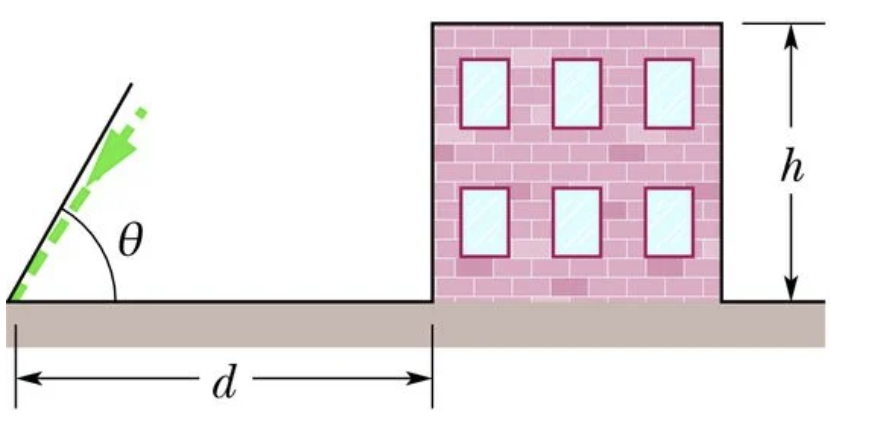
\includegraphics[scale=0.5]{2021-W3-Q3}
\end{figure}

%\section*{Problem 4}
%
%$k=9$\\
%$\vect{A} = 2\unitvect{i} + 4\unitvect{j} + 6\unitvect{k}$\\
%$\vect{B} = 4\unitvect{i} -20\unitvect{j} + 12\unitvect{k}$\\
%$\vect{C} =  \unitvect{i} -10\unitvect{j} - 3\unitvect{k}$. \\[1ex]
%What is $k\vect{A}\cdot (\vect{B}\times\vect{C})$?
%
%\iftoggle{answers}{
%\vspace{1cm}
%\noindent
%SOLUTION:\\
%
%}{}

\section*{Want more practice?}

Further problems on projectiles: Chapter 4.4 problems 21-55\\
Further problems on UCM: Chapter 4.5 problems 56-68\\
\end{document}





 




 


